\documentclass{standalone}

\usepackage{pgfplots}
\usetikzlibrary{decorations.text,positioning,3d,shapes.geometric}

\begin{document}

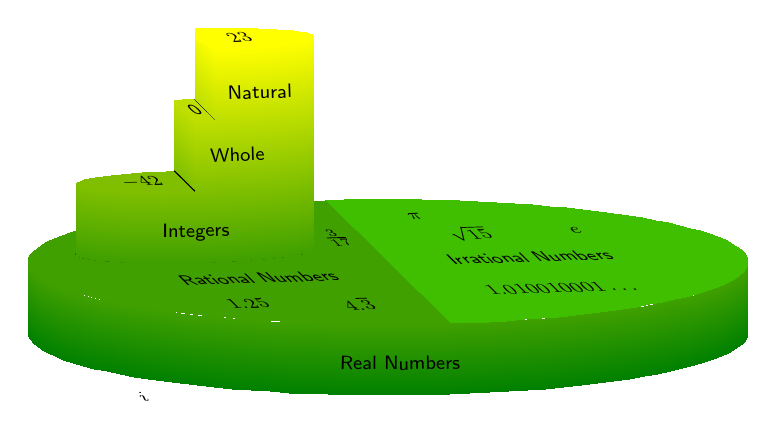
\begin{tikzpicture}
                            \sffamily\scriptsize
                            \def\h{80}% horizontal viewing angle
                            \def\v{10}% vertical viewing angle
                            \begin{axis}[
                                axis lines=none,
                                scale mode=scale uniformly,
                                view={\h}{\v},
                                clip=false,
                                xmin=0,xmax=1,
                                ymin=0,ymax=1,
                                zmin=0,zmax=1,
                                colormap={irrational}{rgb=(0,1,0) rgb=(1,0,0)}
                            ]
                                \path (axis cs:0.9,-0.9,0) -- (axis cs:0.9,-0.8,0) node[midway,sloped,xslant=tan(\a+\b+90),yscale=sin(\a+\b)] {$i$};
                                %Real Wall      
                                \addplot3[domain=90:-100, smooth, surf, shader=interp, y domain=0:0.2, colormap/greenyellow, samples=60, samples y=2] ({cos(x)},{sin(x)},{y});
                                \addplot3[decorate,decoration={text along path,text align=center,text={Real Numbers}},domain=-90:90] ({cos(x)},{sin(x)},{0.07});
                                %Irrational Ceiling                 
                                \addplot3[domain=0:180, smooth, surf, shader=interp, y domain=0:1, colormap name={irrational}, samples=60, samples y=2] ({y*cos(x)},{y*sin(x)},{0.2});
                                \path (axis cs:0,0,0.2) -- (axis cs:0,0.8,0.2) node[midway,sloped,xslant=tan(\a+\b+90),yscale=sin(\a+\b)] {Irrational Numbers};
                                \path (axis cs:-0.7,0,0.2) -- (axis cs:-0.7,0.4,0.2) node[midway,sloped,xslant=tan(\a+\b+90),yscale=sin(\a+\b)] {$\pi$};
                                \path (axis cs:-0.4,0,0.2) -- (axis cs:-0.4,0.6,0.2) node[midway,sloped,xslant=tan(\a+\b+90),yscale=sin(\a+\b)] {$\sqrt{15}$};
                                \path (axis cs:-0.4,0.3,0.2) -- (axis cs:-0.4,0.9,0.2) node[midway,sloped,xslant=tan(\a+\b+90),yscale=sin(\a+\b)] {$e$};
                                \path (axis cs:0.5,0,0.2) -- (axis cs:0.5,0.8,0.2) node[midway,sloped,xslant=tan(\a+\b+90),yscale=sin(\a+\b)] {$1.010010001\ldots$};
                                %Rational Ceiling
                                \addplot3[domain=180:360, smooth, surf, shader=interp, y domain=0:1, colormap/greenyellow, samples=60, samples y=2] ({y*cos(x)},{y*sin(x)},{0.2});
                                \path (axis cs:0.2,-0.8,0.2) -- (axis cs:0.2,0,0.2) node[midway,sloped,xslant=tan(\a+\b+90),yscale=sin(\a+\b)] {Rational Numbers};
                                \path (axis cs:0.6,-0.7,0.2) -- (axis cs:0.6,-0.3,0.2) node[midway,sloped,xslant=tan(\a+\b+90),yscale=sin(\a+\b)] {$1.25$};
                                \path (axis cs:0.65,-0.4,0.2) -- (axis cs:0.65,0,0.2) node[midway,sloped,xslant=tan(\a+\b+90),yscale=sin(\a+\b)] {$4.\overline{3}$};
                                \path (axis cs:-0.4,-0.15,0.2) -- (axis cs:-0.4,0,0.2) node[midway,sloped,xslant=tan(\a+\b+90),yscale=sin(\a+\b)] {$\frac{3}{17}$};
                                %Integer Wall
                                \addplot3[domain=-100:90, thin, samples=60] ({cos(x)/6-1/4},{sin(x)/3-1/2},{0.2});                 
                                \addplot3[domain=90:-100, smooth, surf, shader=interp, y domain=0.2:0.4, colormap/greenyellow, samples=60, samples y=2] ({cos(x)/6-1/4},{sin(x)/3-1/2},{y});
                                \addplot3[decorate,decoration={text along path,text align=center,text={Integers}},domain=-90:90] ({cos(x)/6-1/4},{sin(x)/3-1/2},{0.27});
                                %Integer Ceiling
                                \addplot3[domain=0:360, smooth, surf, shader=interp, y domain=0:1, colormap/greenyellow, samples=60, samples y=2] ({y*cos(x)/6-1/4},{y*sin(x)/3-1/2},{0.4});
                                \path (axis cs:-0.25,-0.8,0.4) -- (axis cs:-0.25,-0.5,0.4) node[midway,sloped,xslant=tan(\a+\b+90),yscale=sin(\a+\b)] {$-42$};
                                %Whole Wall
                                \addplot3[domain=90:-5, smooth, surf, shader=interp, y domain=0.4:0.6, colormap/greenyellow, samples=60, samples y=2] ({cos(x)/6-1/4},{sin(x)/3-1/2},{y});
                                \addplot3[domain=-1:1, smooth, surf, shader=interp, y domain=0.4:0.6, colormap/greenyellow, samples=2, samples y=2] ({x/6*cos(-5)-1/4},{sin(-5)/3-1/2},{y});
                                \addplot3[domain=-1:1, samples=2] ({x/6*cos(-5)-1/4},{sin(-5)/3-1/2},{0.4});
                                \addplot3[decorate,decoration={text along path,text align=center,text={Whole}},domain=-5:40] ({1/6-1/4-0.06},{x*3.1415926/180/3-1/2},{0.47});
                                %Whole Ceiling
                                \addplot3[domain=-5:5, smooth, surf, shader=interp, y domain=-1:1, colormap/greenyellow, samples=60, samples y=2] ({y*cos(x)/6-1/4},{sin(x)/3-1/2},{0.6});
                                \path (axis cs:-0.25,-0.6,0.6) -- (axis cs:-0.25,-0.4,0.6) node[midway,sloped,xslant=tan(\a+\b+90),yscale=sin(\a+\b)] {0};
                                \addplot3[domain=-1:1, samples=2] ({x/6*cos(5)-1/4},{sin(5)/3-1/2},{0.6});
                                %Natural Wall
                                \addplot3[domain=90:5, smooth, surf, shader=interp, y domain=0.6:0.8, colormap/greenyellow, samples=60, samples y=2] ({cos(x)/6-1/4},{sin(x)/3-1/2},{y});
                                \addplot3[domain=-1:1, smooth, surf, shader=interp, y domain=0.6:0.8, colormap/greenyellow, samples=2, samples y=2] ({x/6*cos(5)-1/4},{sin(5)/3-1/2},{y});
                                \addplot3[decorate,decoration={text along path,text align=center,text={Natural}},domain=5:50] ({1/6-1/4-0.03},{x*3.1415926/180/3-1/2},{0.65});
                                %Natural Ceiling
                                \addplot3[domain=5:175, smooth, surf, shader=interp, y domain=0:1, colormap/greenyellow, samples=60, samples y=2] ({y*cos(x)/6-1/4},{y*sin(x)/3-1/2},{0.8});
                                \path (axis cs:-0.25,-0.75,0.8) -- (axis cs:-0.25,0,0.8) node[midway,sloped,xslant=tan(\a+\b+90),yscale=sin(\a+\b)] {$23$};
                                \pgfmathparse{atan(tan(\h)*sin(\v))}
                                \let\a=\pgfmathresult
                                \pgfmathparse{atan(tan(90-\h)*sin(\v))}
                                \let\b=\pgfmathresult  
                            \end{axis}
                        \end{tikzpicture}
\end{document}